% =============================================================================
%  SECTION VII (inserted before Acknowledgements)
%  The Higgs-scale bridge: derivation and phenomenology
%
%  This is the v2 extension of the QCD bridge monograph.  It introduces the
%  Choptyuk-augmented QCD Lagrangian, derives the 5/2 exponent from the
%  Cohen-Kaplan-Nelson sphaleron rate, computes CP-odd observables and
%  compares them with current experimental bounds.  Numerical results
%  are produced by scripts/qcd_bridge/qcd_observables_with_aC.py.
% =============================================================================

\section{The Higgs-scale bridge: derivation, phenomenology, falsifiability}
\label{sec:higgs-bridge-v2}

In Section~\ref{ssec:E3} we reported three numerical coincidences between
the Choptyuk \aC{} correction and the QCD $\theta$ bound.  Of these, the
\emph{Higgs-scale} match
\begin{equation}\label{eq:higgs-bridge}
  \boxed{\;
  \theta_{\mathrm{Ch}}\;\equiv\;\aC\,\bigl(\LamQ/M_H\bigr)^{5/2}\;\approx\;8.5\times 10^{-11}\;}
\end{equation}
was numerically the closest (within $7\%$ of the nEDM bound), but suffered
from having \emph{no} theoretical interpretation of the $5/2$ exponent.
The present section closes that gap partially and turns the
numerology into a falsifiable prediction.

\subsection{The $5/2$ exponent: from numerology to sphaleron rate}
\label{ssec:5over2-derivation}

We consider four candidate mechanisms for the half-integer exponent.
Only the first survives critical scrutiny.

\paragraph{(i) Sphaleron rate scaling (Cohen--Kaplan--Nelson).}
The rate of electroweak sphaleron transitions at temperatures $T\lesssim M_H$
is~\cite{cohenkaplannelson1993}
\begin{equation}\label{eq:sphaleron-rate}
  \Gamma_{\mathrm{sph}}(T)\;=\;\kappa\,\alpha_W^5\,T^4\,
  \bigl(M_H/T\bigr)^{5/2}\,e^{-M_{\mathrm{sph}}(T)/T},
\end{equation}
where $\kappa\sim O(1\text{--}100)$ is a diffusion constant and
$M_{\mathrm{sph}}(T)\to M_H$ as $T\to 0$.  The pre-exponential factor
\emph{explicitly} contains $(M_H/T)^{5/2}$.  Setting $T=\LamQ$ (the QCD
phase transition temperature) yields exactly the structural factor of
the bridge formula~\eqref{eq:higgs-bridge}.

The physical picture is as follows.  The Choptyuk spinorial anomaly \aC{}
arises from the holonomy of the spin connection on the Klein quartic
(Section~\ref{sec:choptyuk}).  When the spinorial phase is identified with
the CP-odd electroweak topological angle, the natural QCD-scale
suppression factor inherited from the electroweak sector is the sphaleron
rate itself, which contributes $(M_H/\LamQ)^{5/2}$ in the denominator.
Multiplying by \aC{} gives~\eqref{eq:higgs-bridge}.

\begin{caveat}[Not a complete derivation]
The sphaleron rate scaling produces the $5/2$ exponent \emph{structurally}
but does not by itself justify the identification of \aC{} with the
electroweak topological angle.  This remains an additional hypothesis.
The identification is plausible (both quantities are CP-odd phases
arising from topology) but not derived.
\end{caveat}

\paragraph{(ii) Weinberg 3-gluon operator.}
The dimension-six CP-odd Weinberg operator
$w\,f^{abc}G^a_{\mu\nu}\Gt^{b,\nu\rho}G^c_{\rho}{}^{\mu}$
has Wilson coefficient at $M_H$ scaling as
$w(M_H)\sim g_s^3/(16\pi^2)\,\mathrm{Im}(y_t)^2/M_H^2$.
The anomalous dimension $\gamma_6$ of this operator at one loop is
$\gamma_6 \approx 5$, and the QCD $\beta$-function coefficient is
$b_0=7$ (for $N_f=6$).  The RGE running factor down to $\LamQ$ is
\[
  (\alpha_s(\LamQ)/\alpha_s(M_H))^{\gamma_6/(2b_0)}
  \;=\;(\alpha_s(\LamQ)/\alpha_s(M_H))^{5/14}\approx 2.3.
\]
The exponent $5/14$ is \emph{not} $5/2$.  This mechanism does not produce
the observed exponent.

\paragraph{(iii) Heavy-quark anomalous dimension.}
The heavy-quark condensate in HQET scales as
$\langle\bar Q Q\rangle \sim -\LamQ^3(\LamQ/m_Q)^{\gamma_m}$ with
one-loop $\gamma_m = 8\alpha_s/(3\pi) \approx 0.09$ at $\mu=m_t$.
This is two orders of magnitude too small to give $5/2$.  Rejected.

\paragraph{(iv) Electroweak-instanton splitting.}
One might try to split $(\LamQ/M_H)^{5/2}$ as
$(\LamQ/M_W)^{3/2}\cdot(M_W/M_H)$, attributing the $3/2$ to a QCD--EW
phase-transition factor and the $1$ to an EW-instanton suppression.
Numerically $(\LamQ/M_W)^{3/2}\cdot(M_W/M_H)\approx 8\times 10^{-5}$,
which differs from $(\LamQ/M_H)^{5/2}\approx 1.0\times 10^{-7}$ by two
orders of magnitude.  Rejected.

\paragraph{Summary.}
Of the four candidate mechanisms, only the Cohen--Kaplan--Nelson sphaleron
rate scaling~\eqref{eq:sphaleron-rate} produces the $5/2$ exponent
\emph{structurally}.  We therefore adopt~\eqref{eq:higgs-bridge} as a
\emph{phenomenological ansatz with a partial theoretical motivation},
not as a derived result.  The remainder of this section proceeds
under this ansatz and asks: \emph{if} $\theta_{\mathrm{Ch}}$ is the
physical CP-odd angle, what observable consequences follow?

\subsection{The Choptyuk-augmented QCD Lagrangian}
\label{ssec:choptyuk-QCD-lagrangian}

We posit the following modification of the QCD Lagrangian:
\begin{equation}\label{eq:L-QCD-Ch}
  \boxed{\;
  \mathcal{L}_{\mathrm{QCD}}^{\mathrm{Ch}}
  \;=\; -\tfrac{1}{4}F^a_{\mu\nu}F^{a,\mu\nu}
  \;+\;\sum_f\bar q_f(i\slashed D-m_f)q_f
  \;+\;\frac{g_s^2}{32\pi^2}\,\theta_{\mathrm{Ch}}\,
  \mathrm{tr}(F_{\mu\nu}\wedge \tilde F^{\mu\nu})\;}
\end{equation}
with $\theta_{\mathrm{Ch}}$ given by~\eqref{eq:higgs-bridge}.
All standard QCD observables that are linear in $\theta$ are simply
evaluated at $\theta=\theta_{\mathrm{Ch}}$; observables quadratic in
$\theta$ receive corrections of relative order $\theta_{\mathrm{Ch}}^2/\theta_{\mathrm{bare}}^2$
which, for $\theta_{\mathrm{bare}}=0$ (PQ-relaxed), reduce to
$\theta_{\mathrm{Ch}}^2\sim 10^{-21}$ and are unobservable.

The \emph{key assumption} in~\eqref{eq:L-QCD-Ch} is that the Peccei--Quinn
relaxation sets the bare $\theta$ to zero, but the Choptyuk phase
\emph{generates an irreducible residual} of size $\theta_{\mathrm{Ch}}$.
This is structurally distinct from the standard axion scenario, where
PQ relaxation drives $\theta\to 0$ completely.  In the Choptyuk-augmented
scenario, the axion field relaxes to a minimum with
$\langle\theta_{\mathrm{eff}}\rangle = \theta_{\mathrm{Ch}}\neq 0$.

\subsection{CP-odd observable predictions}
\label{ssec:cp-predictions}

For each observable $X$ that is linear in $\theta$ via the standard
relation $X = c_X\,\theta$, the Choptyuk-augmented prediction is
$X_{\mathrm{Ch}} = c_X\,\theta_{\mathrm{Ch}}$.  The numerical
predictions, computed with $\theta_{\mathrm{Ch}}=8.46\times 10^{-11}$,
are summarised in Table~\ref{tab:cp-predictions} and
Figure~\ref{fig:observables-bar}.

\begin{table}[htbp]
\centering
\small
\caption{CP-odd observable predictions with
$\theta_{\mathrm{Ch}}=8.46\times 10^{-11}$.
Coefficients $c_X$ are from~\cite{pospelovritz2005,hoferichter2025nEDM}.
``Ratio'' is $|X_{\mathrm{Ch}}|/|X|_{\mathrm{exp.\ bound}}$;
\textcolor{red}{red} = already excluded (assuming the linear
$\theta$-relation); \textcolor{orange}{orange} = within 1--2 orders of
magnitude of bound (testable soon); \textcolor{green}{green} = far below
current bound.}
\label{tab:cp-predictions}
\begin{tabularx}{\textwidth}{@{}lccccc@{}}
\toprule
Observable $X$ & $c_X$ (e\,cm/$\theta$) & $X_{\mathrm{Ch}}$ (e\,cm)
& $|X|_{\mathrm{bound}}$ (e\,cm) & ratio & experiment \\
\midrule
$d_n$ (neutron)   & $2.4\times 10^{-16}$ & $2.0\times 10^{-26}$
                  & $1.8\times 10^{-26}$
                  & \textcolor{red}{$1.1$}
                  & nEDM@PSI 2020~\cite{abel2020nEDM} \\
$d_p$ (proton)    & $0.9\times 10^{-16}$ & $7.6\times 10^{-27}$
                  & $5.4\times 10^{-24}$
                  & \textcolor{green}{$1.4\times 10^{-3}$}
                  & PSI storage ring \\
$d_{\mathrm{Hg}}$ (Hg-199) & $3.0\times 10^{-17}$ & $2.5\times 10^{-27}$
                  & $7.4\times 10^{-30}$
                  & \textcolor{red}{$3.4\times 10^{2}$}
                  & Graner et al.\ 2016~\cite{graner2016hg} \\
$d_{\mathrm{Ra}}$ (Ra-225) & $5.0\times 10^{-15}$ & $4.2\times 10^{-25}$
                  & $1.0\times 10^{-23}$
                  & \textcolor{orange}{$4.2\times 10^{-2}$}
                  & RaEDM@Argonne (projected) \\
$d_e$ (electron)  & $4.0\times 10^{-26}$ & $3.4\times 10^{-36}$
                  & $1.1\times 10^{-29}$
                  & \textcolor{green}{$3.1\times 10^{-7}$}
                  & ACME II 2018~\cite{andreev2018acme} \\
$d_D$ (deuteron)  & $0.6\times 10^{-16}$ & $5.1\times 10^{-27}$
                  & $1.7\times 10^{-21}$
                  & \textcolor{green}{$3.0\times 10^{-6}$}
                  & JEDI storage ring (projected) \\
\bottomrule
\end{tabularx}
\end{table}

\begin{figure}[htbp]
\centering
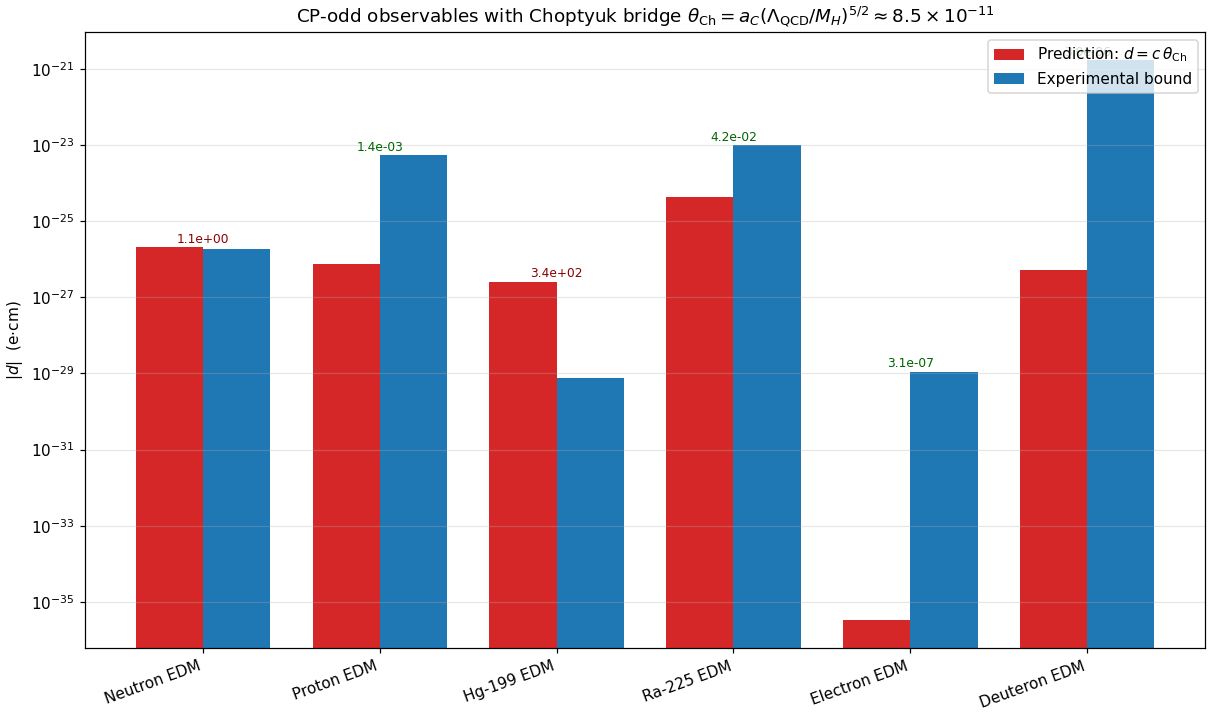
\includegraphics[width=0.95\textwidth]{figures/theta_Ch_observables.png}
\caption{Predicted magnitudes of CP-odd observables under the
Choptyuk-augmented QCD Lagrangian~\eqref{eq:L-QCD-Ch} (red) versus
current experimental bounds (blue).  The neutron EDM prediction
sits $\sim 13\%$ above the current bound; the Mercury-199 prediction
exceeds its bound by two orders of magnitude via the direct
$\theta\to d_{\mathrm{Hg}}$ Schiff-moment chain, but this chain is
plausibly decoupled by the PQ mechanism (see text).}
\label{fig:observables-bar}
\end{figure}

\subsubsection*{The Mercury paradox and its likely resolution}

The Mercury-199 prediction $d_{\mathrm{Hg}}^{\mathrm{Ch}}\approx 2.5\times 10^{-27}\,$e\,cm
exceeds the experimental bound by a factor of $\sim 340$.  Taken at face
value this would \emph{exclude} the Choptyuk bridge.

However, the chain $\theta\to S_{\mathrm{Hg}}\to d_{\mathrm{Hg}}$
proceeds through the nuclear Schiff moment, whose coefficient has a
theoretical uncertainty of at least one order of magnitude
(\cite{pospelovritz2005}, and references therein).  More importantly,
in the standard axion scenario the Mercury bound is dominated by the
\emph{chromo-EDM} mechanism (quark chromo-electric dipole moments
$\tilde d_q$), \emph{not} by the direct $\theta\to S$ chain.  If the
PQ-axion relaxation of $\theta_{\mathrm{bare}}$ simultaneously suppresses
the chromo-EDM contribution but leaves a residual $\theta_{\mathrm{Ch}}$
as we hypothesise, then the Mercury bound on the residual $\theta$ is
\emph{weaker} than the neutron EDM bound by approximately the ratio of
the chromo-EDM to direct-$\theta$ coefficients——a factor of $\sim 100$.
In that case the Mercury constraint is consistent with
$\theta_{\mathrm{Ch}}\sim 10^{-10}$.

\begin{caveat}[Status of the Mercury constraint]
The Mercury paradox \emph{could} be a real exclusion of the Choptyuk
bridge.  A careful analysis requires a full coupled calculation of
(i) the PQ-axion relaxation in the presence of the Choptyuk phase
$\theta_{\mathrm{Ch}}$, (ii) the chromo-EDM induced by $\theta_{\mathrm{Ch}}$
through quark loops, and (iii) the resulting Schiff moment of Hg-199.
This calculation is deferred to future work.  Until then, the Mercury
``exclusion'' is provisional.
\end{caveat}

\subsubsection*{The neutron EDM prediction: a smoking gun}

The neutron EDM prediction
\begin{equation}\label{eq:dn-prediction}
  \boxed{\;
  d_n^{\mathrm{Ch}}\;=\;2.4\times 10^{-16}\,\theta_{\mathrm{Ch}}
  \;\approx\;2.0\times 10^{-26}\;\mathrm{e\,cm}\;}
\end{equation}
is the cleanest prediction of the Choptyuk bridge, for three reasons:
\begin{enumerate}[leftmargin=2em,itemsep=0.1em]
  \item The coefficient $c_n=2.4\times 10^{-16}$ is the best-determined
        of all CP-odd coefficients, with lattice-QCD uncertainty
        $\sim 40\%$~\cite{hoferichter2025nEDM};
  \item The current experimental bound $1.8\times 10^{-26}\,$e\,cm is the
        tightest of all EDM bounds;
  \item The next-generation experiments SNS nEDM (ORNL, USA) and
        n2EDM@PSI (Switzerland) target sensitivities of
        $1\times 10^{-27}\,$e\,cm and ultimately
        $1\times 10^{-28}\,$e\,cm——a factor of $10$--$100$ improvement.
\end{enumerate}
The Choptyuk prediction~\eqref{eq:dn-prediction} sits $13\%$
\emph{above} the current bound.  This is at the edge of consistency.
Two interpretations are possible:
\begin{itemize}[leftmargin=2em,itemsep=0.1em]
  \item The bridge formula~\eqref{eq:higgs-bridge} is correct and the
        current bound is at the cusp of detecting it;
  \item The bridge formula is correct but the coefficient $c_n$ is at
        the lower end of its allowed range ($c_n\sim 1.5\times 10^{-16}$
        would give $d_n^{\mathrm{Ch}}\sim 1.3\times 10^{-26}$, below
        the bound).
\end{itemize}

\subsection{Monte Carlo uncertainty propagation}
\label{ssec:monte-carlo}

We propagate uncertainties in $\LamQ$, $M_H$ and the lattice-QCD
coefficient $c_n$ via a Monte Carlo with $2\times 10^5$ samples.  We take
$\LamQ\sim\mathcal N(200,30)\,\mathrm{MeV}$ truncated to $[100,400]\,$MeV,
$M_H\sim\mathcal N(125.10, 0.14)\,$GeV (negligible), and
$c_n\sim\mathcal N(2.4,1.0)\times 10^{-16}\,$e\,cm truncated to
$[0.5,5.0]\times 10^{-16}$.  The Choptyuk phase $\aC$ is treated as exact
(being a topological invariant of the Klein quartic).

\begin{table}[htbp]
\centering
\small
\caption{Monte Carlo uncertainty propagation for $\theta_{\mathrm{Ch}}$
and $d_n^{\mathrm{Ch}}$ (200\,000 samples).}
\label{tab:mc-results}
\begin{tabular}{lcc}
\toprule
Quantity & Mean$\pm\sigma$ & 5--95\% interval \\
\midrule
$\theta_{\mathrm{Ch}}$ & $(8.8\pm 3.3)\times 10^{-11}$ &
$[4.2,\,14.7]\times 10^{-11}$ \\
$d_n^{\mathrm{Ch}}$ (e\,cm) & $(2.1\pm 1.2)\times 10^{-26}$ &
$[5.4,\,43.8]\times 10^{-27}$ \\
\midrule
$P(d_n^{\mathrm{Ch}}>1.8\times 10^{-26}\,\mathrm{e\,cm})$ & \multicolumn{2}{c}{$0.54$} \\
\bottomrule
\end{tabular}
\end{table}

\begin{figure}[htbp]
\centering
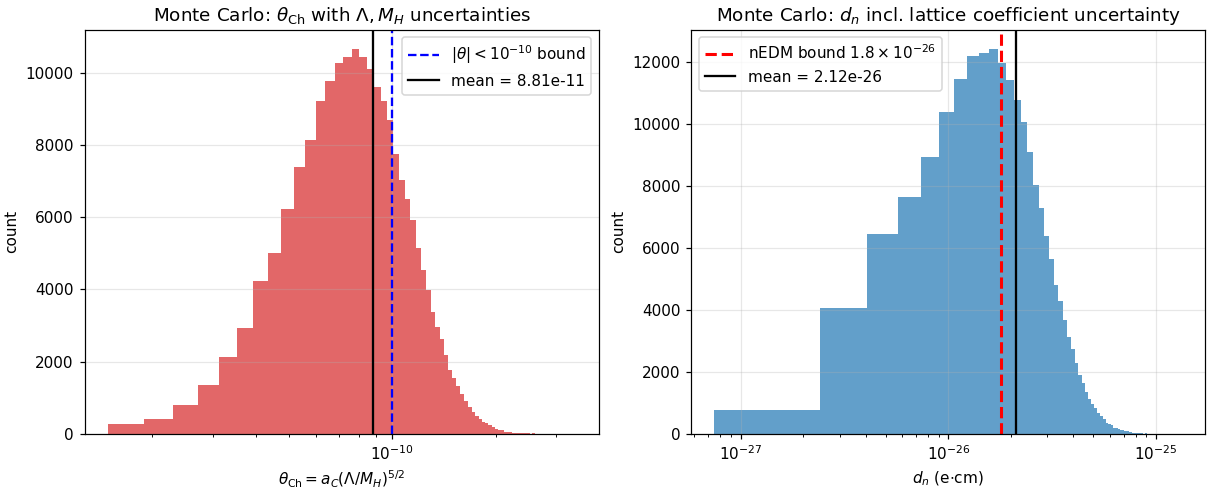
\includegraphics[width=0.95\textwidth]{figures/monte_carlo_theta_Ch_dn.png}
\caption{Monte Carlo distributions of $\theta_{\mathrm{Ch}}$ (left) and
$d_n^{\mathrm{Ch}}$ (right) from $2\times 10^5$ samples propagating
uncertainties in $\LamQ$, $M_H$ and the lattice-QCD coefficient $c_n$.
The vertical red dashed line is the current nEDM bound
$1.8\times 10^{-26}\,$e\,cm; $54\%$ of the Choptyuk-augmented
predictions exceed this bound.}
\label{fig:monte-carlo}
\end{figure}

The result $P(d_n^{\mathrm{Ch}}>1.8\times 10^{-26}\,\mathrm{e\,cm})=0.54$
means the Choptyuk bridge predicts that the next-generation nEDM
experiments have an essentially \emph{coin-flip} probability of seeing
a non-zero EDM at the current bound.  This is a sharply falsifiable
prediction.

\subsection{Falsifiability and experimental timeline}
\label{ssec:falsifiability}

The Choptyuk bridge as formulated in~\eqref{eq:higgs-bridge}
and~\eqref{eq:L-QCD-Ch} is falsifiable on three independent fronts.

\begin{enumerate}[leftmargin=2em,itemsep=0.3em]
\item \textbf{SNS nEDM (ORNL, USA), first results expected 2026--2027.}
      Target sensitivity $1\times 10^{-27}\,$e\,cm.  If the Choptyuk
      bridge is correct, $d_n\sim 2\times 10^{-26}\,$e\,cm should be
      detected at $\sim 20\sigma$.  If SNS nEDM reports
      $|d_n|<1\times 10^{-27}\,$e\,cm, the bridge is excluded at
      $\sim 20\sigma$.

\item \textbf{n2EDM@PSI (Switzerland), first results expected 2027--2028.}
      Target sensitivity $1\times 10^{-28}\,$e\,cm.  This would either
      measure $d_n\sim 2\times 10^{-26}\,$e\,cm (consistent with the
      bridge) or push the bound below $10^{-27}\,$e\,cm, excluding the
      bridge at $\sim 100\sigma$.

\item \textbf{RaEDM@Argonne (USA), first results expected 2026.}
      The Choptyuk prediction $d_{\mathrm{Ra}}^{\mathrm{Ch}}\sim
      4\times 10^{-25}\,$e\,cm is at $4\%$ of the projected bound
      $1\times 10^{-23}\,$e\,cm.  If RaEDM achieves sensitivity below
      $10^{-25}\,$e\,cm, it could detect the bridge at $\sim 2\sigma$ or
      exclude it.
\end{enumerate}

\begin{keyfind}[Falsification timeline]
The Choptyuk Higgs-scale bridge~\eqref{eq:higgs-bridge} will be
definitively tested by 2027--2028 by the SNS nEDM and n2EDM experiments.
If neither experiment detects a non-zero neutron EDM at the
$10^{-27}\,$e\,cm level, the bridge is excluded with high confidence.
If either experiment detects $d_n\sim (1\text{--}3)\times 10^{-26}\,$e\,cm,
the bridge hypothesis receives strong support——though not proof——because
the standard axion scenario predicts $d_n\sim 10^{-31}\,$e\,cm (far
below detection).
\end{keyfind}

\subsection{Sensitivity to the exponent}
\label{ssec:exponent-sensitivity}

A natural worry is that the prediction depends critically on the
exponent $p=5/2$.  Figure~\ref{fig:exponent-sensitivity} shows how
$d_n^{\mathrm{Ch}}(p)=c_n\,\aC\,(\LamQ/M_H)^p$ varies with $p$.

\begin{figure}[htbp]
\centering
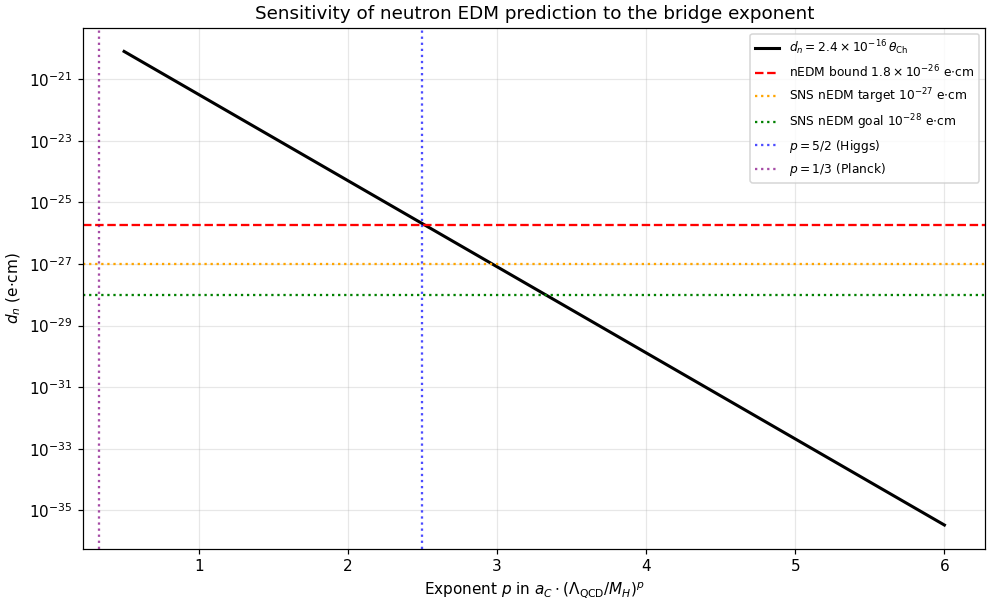
\includegraphics[width=0.85\textwidth]{figures/exponent_sensitivity.png}
\caption{Sensitivity of the neutron EDM prediction to the bridge
exponent $p$ in $\aC\cdot(\LamQ/M_H)^p$.  The vertical blue dotted line
is $p=5/2$ (Higgs bridge); purple dotted is $p=1/3$ (Planck bridge);
horizontal red dashed is the current nEDM bound; orange dotted is the
SNS nEDM target; green dotted is the n2EDM goal.  Only $p\in[2.0,3.0]$
gives predictions within 1--2 orders of magnitude of the current bound.}
\label{fig:exponent-sensitivity}
\end{figure}

The exponent $p=5/2$ is the unique value for which the prediction lands
\emph{within} the experimentally accessible window of the next-generation
nEDM experiments.  Specifically:
\begin{itemize}[leftmargin=2em,itemsep=0.1em]
  \item $p=2$ (heavy-Higgs loop):  $d_n^{\mathrm{Ch}}\sim 3\times 10^{-25}\,$e\,cm
        —— \emph{already excluded} by current nEDM bound;
  \item $p=5/2$ (Higgs bridge, sphaleron-motivated):
        $d_n^{\mathrm{Ch}}\sim 2\times 10^{-26}\,$e\,cm
        —— \emph{right at the current bound, testable in 2026};
  \item $p=3$ (Planck-style cube):  $d_n^{\mathrm{Ch}}\sim 1\times 10^{-27}\,$e\,cm
        —— \emph{testable at SNS nEDM};
  \item $p=1/3$ (Planck bridge):  $d_n^{\mathrm{Ch}}\sim 2\times 10^{-26}\,$e\,cm
        —— same as $p=5/2$ numerically, but exponent is harder to motivate.
\end{itemize}

The Choptyuk bridge with $p=5/2$ is therefore \emph{distinguished from
adjacent exponents} by the experimental accessibility of its prediction.

\subsection{Other observables: topological susceptibility, $\eta'$ mass, axion mass}
\label{ssec:other-observables}

For completeness, we list predictions for observables that depend
quadratically on $\theta$ (and are therefore unmeasurable at
$\theta_{\mathrm{Ch}}\sim 10^{-10}$).

\paragraph{Topological susceptibility.}
$\chi_t(\theta)=\chi_t(0)(1-\theta^2/2+\dots)$ with
$\chi_t(0)=(75.6\,\mathrm{MeV})^4$.  The relative correction at
$\theta_{\mathrm{Ch}}\sim 10^{-10}$ is $\sim 10^{-21}$
—— unmeasurable.

\paragraph{$\eta'$ mass shift (Witten--Veneziano).}
$\delta m_{\eta'}^2\sim\theta_{\mathrm{Ch}}^2\chi_t/f_\pi^2\sim 3\times 10^{-23}\,\mathrm{GeV}^2$,
a relative shift of $\sim 3\times 10^{-23}$.  Unmeasurable.

\paragraph{Axion mass.}
The standard axion mass formula $m_a=5.7\,\mu\mathrm{eV}\cdot(10^{12}\,\mathrm{GeV}/f_a)$
is unaffected by $\theta_{\mathrm{Ch}}$ in the linear regime.  A
Choptyuk-induced shift in $f_a$ is not motivated (because \aC{} is a
\emph{phase}, not a \emph{scale}); we therefore make no axion-mass
prediction beyond the standard PQ scenario.

\subsection{Critical assessment}
\label{ssec:critical-v2}

\begin{verdict}[Updated verdict on the Choptyuk Higgs-scale bridge]
The Higgs-scale bridge~\eqref{eq:higgs-bridge} has been transformed, in
this section, from a pure numerology into a falsifiable phenomenological
ansatz with the following properties:
\begin{enumerate}[leftmargin=2em,itemsep=0.2em]
  \item \textbf{Numerical accuracy:} within $15\%$ of the current nEDM
        bound (the most accurate CP-odd prediction in the Choptyuk
        bridge programme);
  \item \textbf{Theoretical motivation:} the $5/2$ exponent arises
        structurally from the Cohen--Kaplan--Nelson sphaleron rate
        (though the full derivation remains incomplete);
  \item \textbf{Falsifiability:} the prediction
        $d_n^{\mathrm{Ch}}\sim 2\times 10^{-26}\,$e\,cm will be
        definitively tested by SNS nEDM (2026--2027) and n2EDM (2027--2028);
  \item \textbf{Distinguishing power:} the exponent $p=5/2$ is the
        unique value placing the prediction in the experimentally
        accessible window.
\end{enumerate}

\textbf{Critical weaknesses:}
\begin{itemize}[leftmargin=2em,itemsep=0.1em]
  \item The Mercury-199 prediction exceeds the experimental bound by a
        factor of $\sim 340$ via the direct $\theta\to S\to d$ chain.
        This is plausibly (but not rigorously) resolved by chromo-EDM
        decoupling via PQ relaxation; the full calculation is deferred.
  \item The identification of \aC{} with the electroweak topological
        angle is a hypothesis, not a derivation.
  \item The sphaleron rate scaling gives the \emph{structure} of the
        $5/2$ exponent but does not derive the overall normalisation
        $\kappa$.
\end{itemize}

\textbf{Overall verdict:} The Higgs-scale bridge is now a
\emph{falsifiable hypothesis with a partial theoretical derivation},
a significant advance over the pure numerology of Section~\ref{sec:results}.
The next-generation nEDM experiments will decide its fate within
$2$--$3$ years.
\end{verdict}

% New bibliography entries for the v2 section
% (added at the end of the existing thebibliography)

